\section{Transformer}

\subsection{Attention}

我想可能看代码更方便理解, 这是一个非常好的网站 \href{https://nn.labml.ai/transformers/mha.html}{Multi-Headed Attention}

\begin{figure}[htbp]
    \centering
    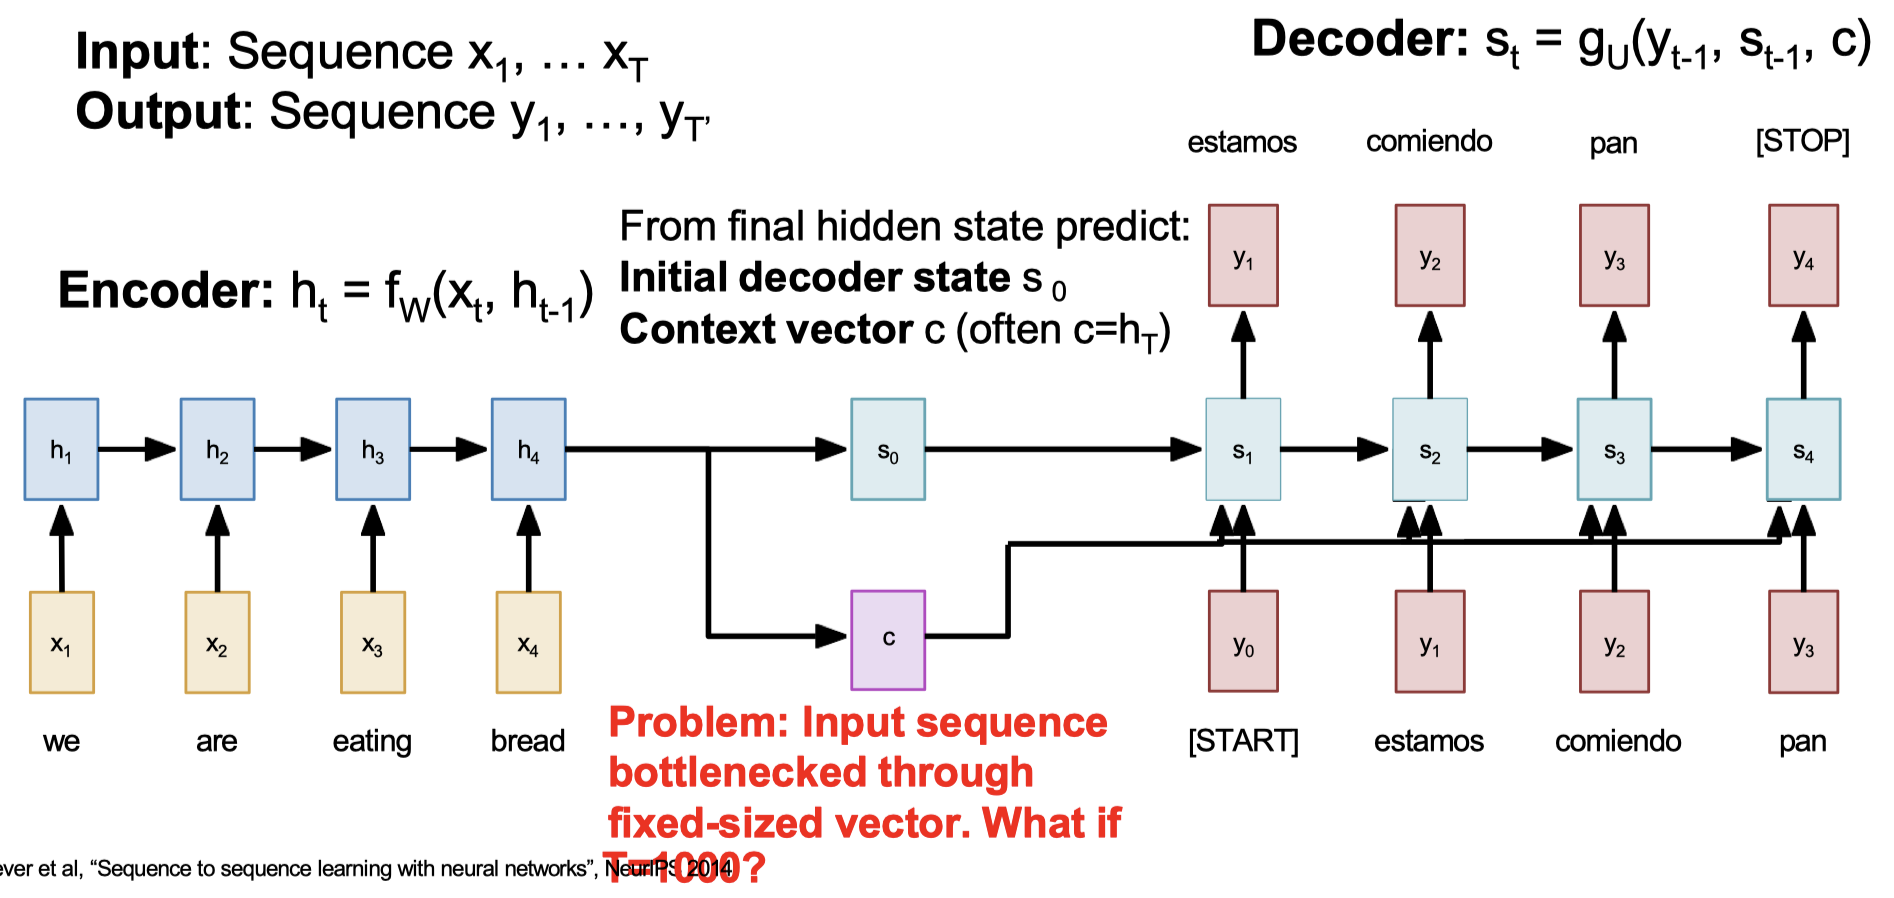
\includegraphics[width=0.8\textwidth]{figures/seq2seq.png}
    \caption{seq2seq}
    \label{fig:seq2seq}
\end{figure}

这样的 c: Context vector 太小了, 无法表达所有句子的信息, 所以考虑使用一个自适应的 Context vector 表达每一个 token 的信息, 这就是 attention 的思想.

\begin{figure}[htbp]
    \centering
    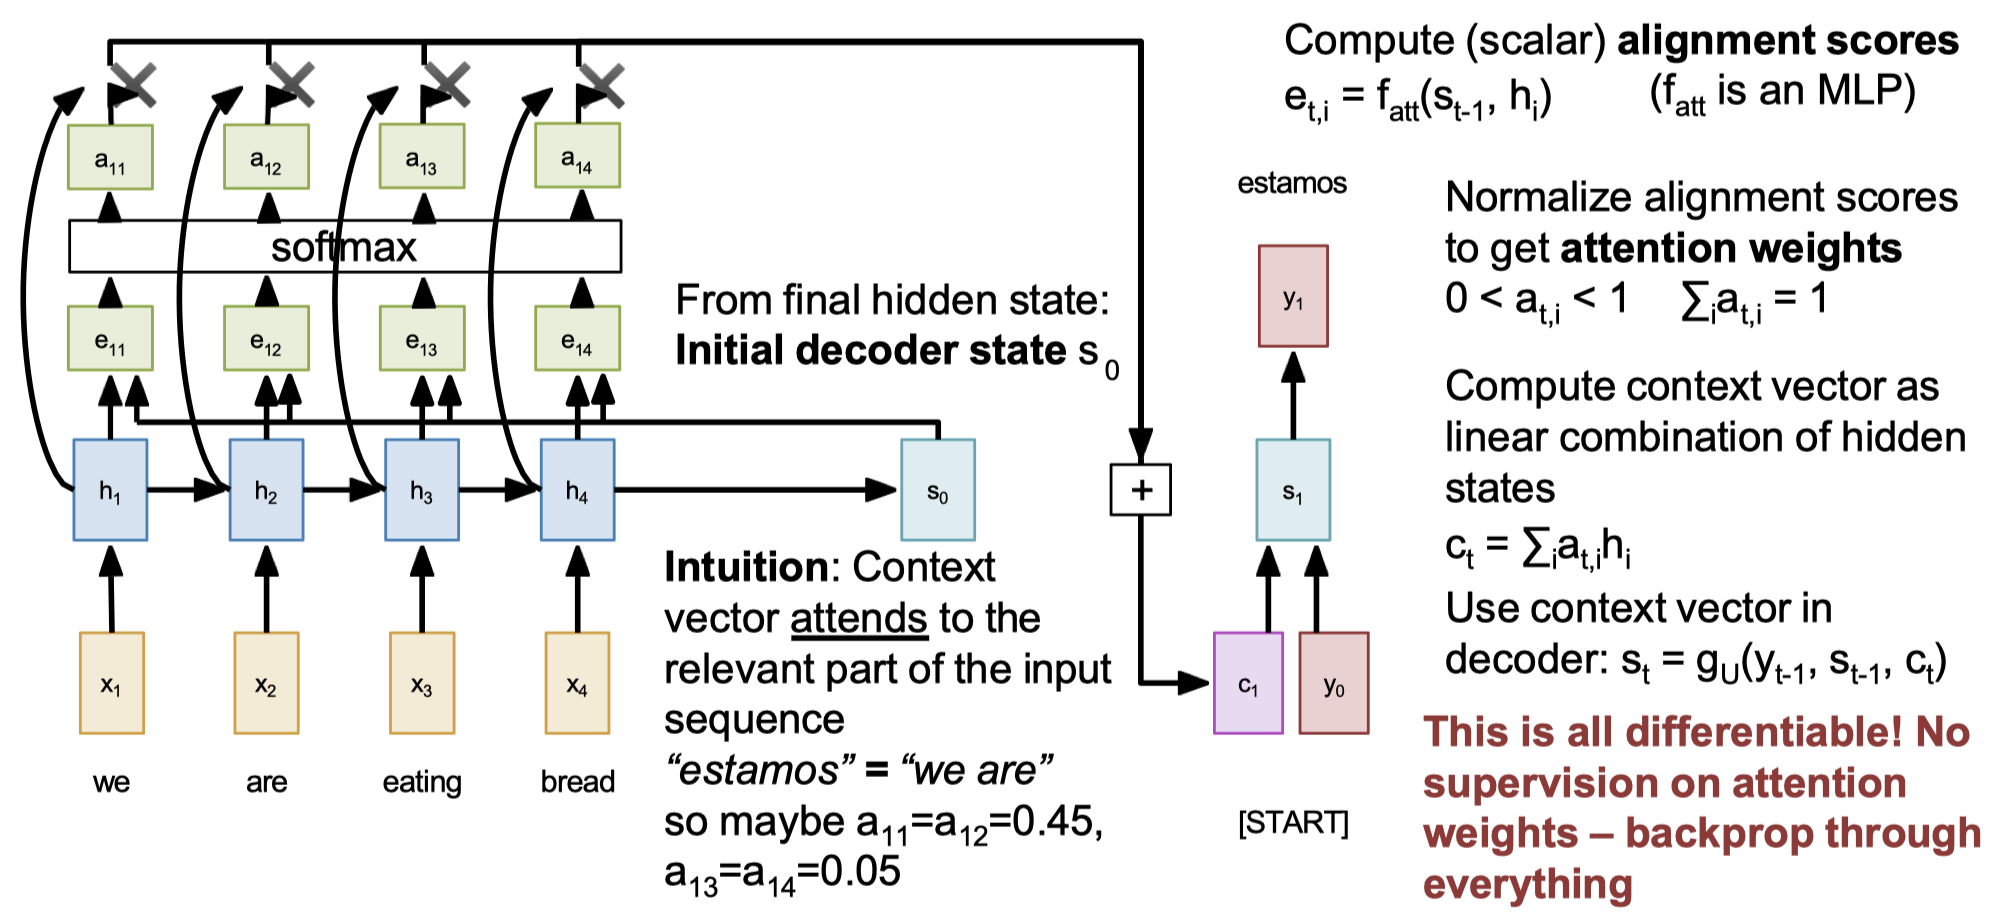
\includegraphics[width=0.8\textwidth]{figures/attention.png}
    \caption{Attention}
    \label{fig:Attention}
\end{figure}

对应到 Transformer 中, Query 是 s, Cross attention 的输出就是 c.

\begin{figure}[htbp]
    \centering
    \includegraphics[width=0.4\textwidth]{figures/Transformer.png}
    \caption{Transformer}
    \label{fig:Transformer}
\end{figure}

如何把 attention 应用到图片中呢? 这和语言中的基本单元类似, 语言中的基本单元在 embedding 后已经不是一个单词了, 而是一个个 token.
考虑把卷积之后的每个像素的所有 feature 看作 token, 然后进行类似结构即可.

\begin{figure}[htbp]
    \centering
    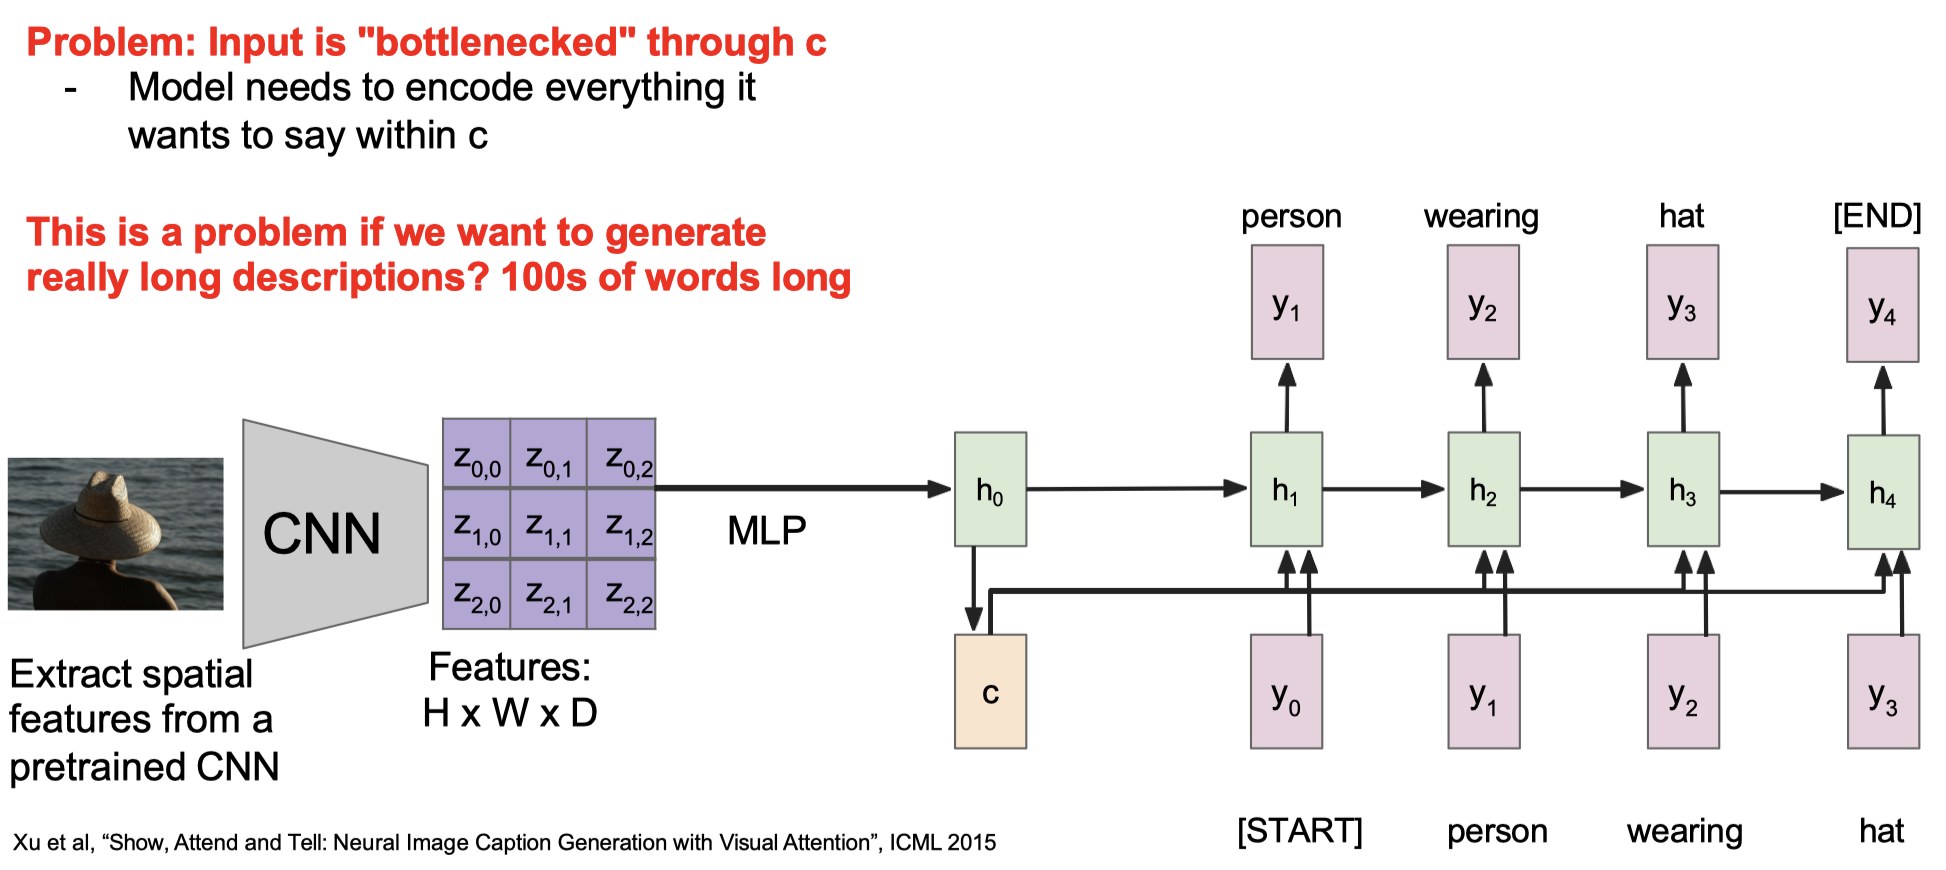
\includegraphics[width=0.8\textwidth]{figures/image_seq2seq.png}
    \caption{Image seq2seq}
    \label{fig:image_seq2seq}
\end{figure}

这里实际上没有使用 attention, 是经典的 seq2seq 模型, 但是可以使用 attention 来改进.

\begin{figure}[htbp]
    \centering
    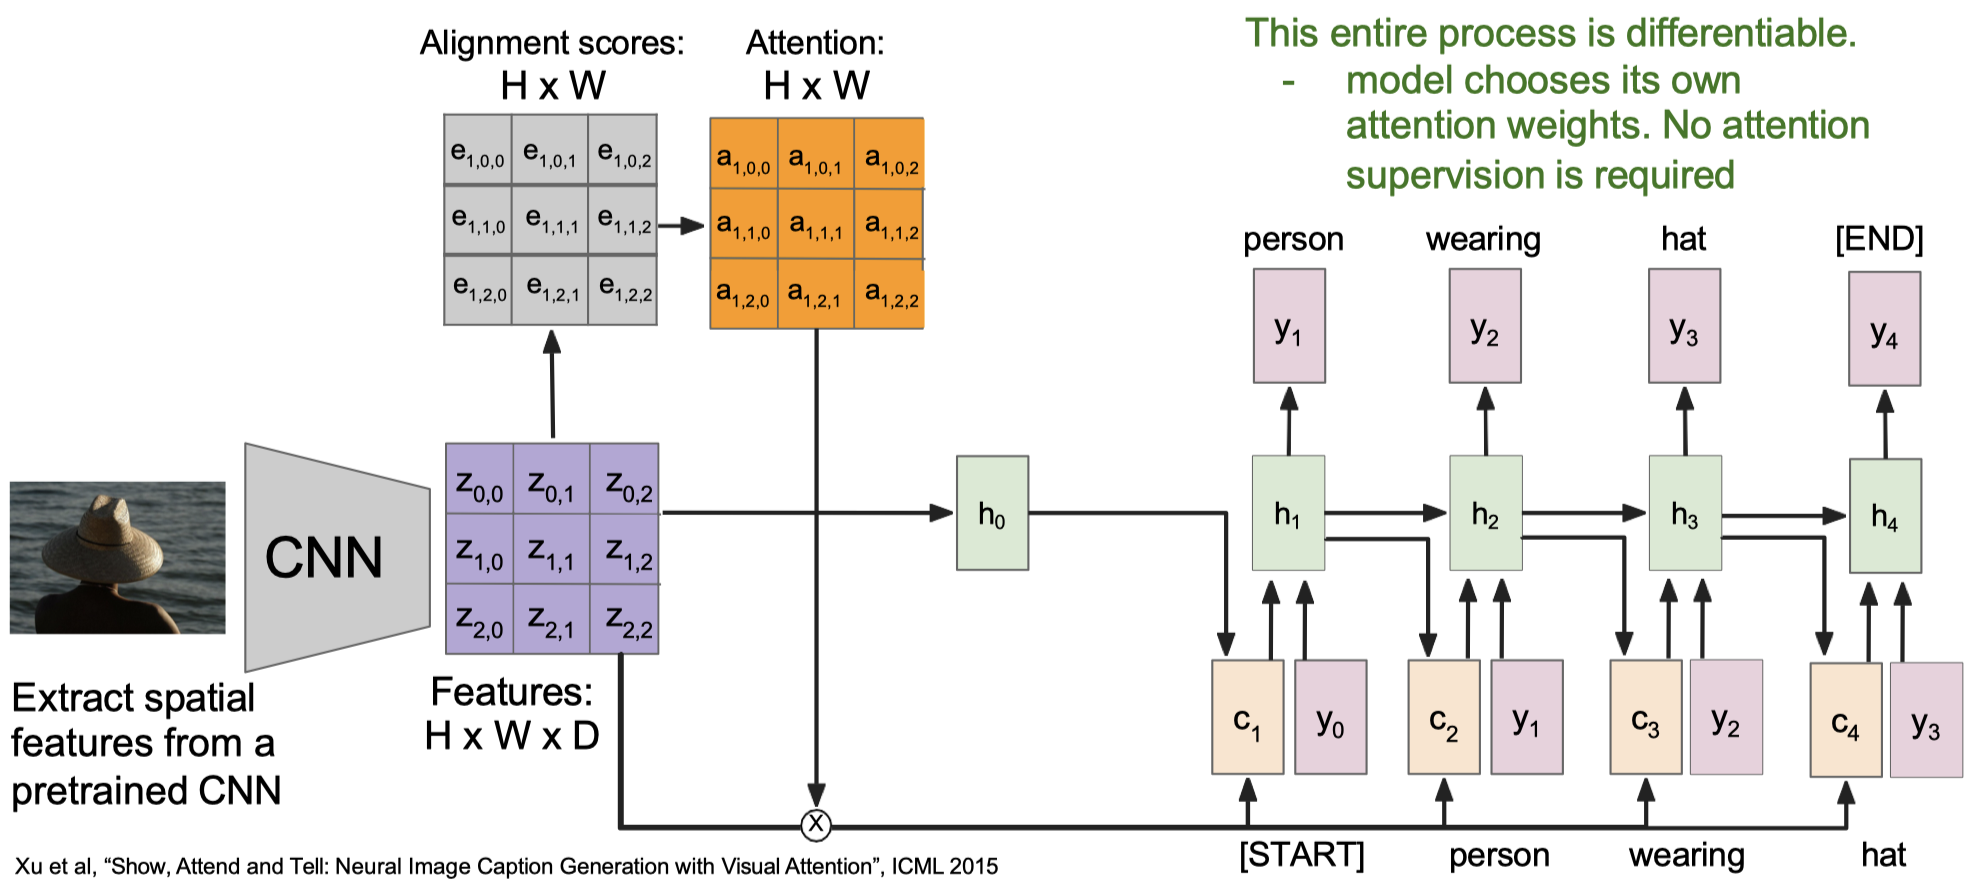
\includegraphics[width=0.8\textwidth]{figures/image_attentoin.png}
    \caption{Image Attention Grad Flow}
    \label{fig:image_attentoin}
\end{figure}

跟NLP中的attention很类似.

一个实现细节: 相似度使用内积还是余弦相似度?取决于有没有对作归一化

\begin{figure}[htbp]
    \centering
    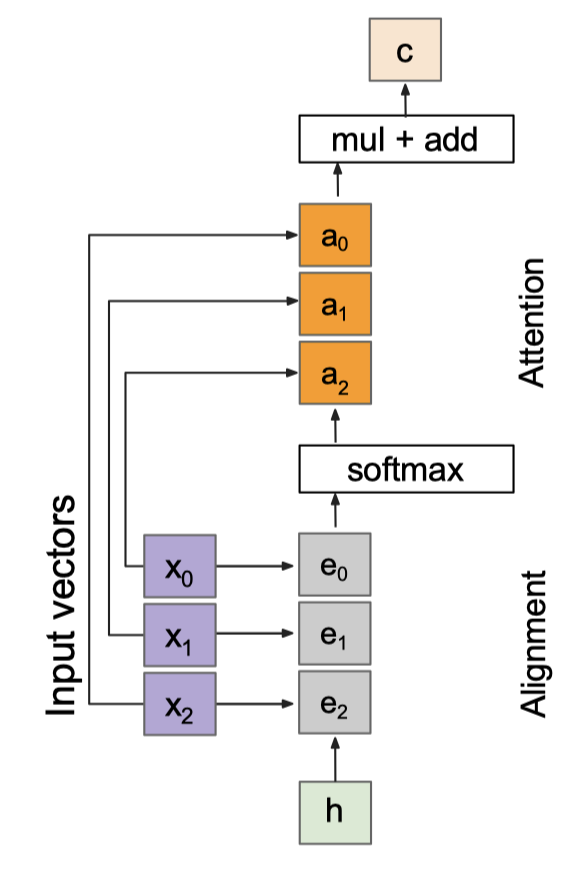
\includegraphics[width=0.4\textwidth]{figures/general_atten.png}
    \caption{General Attention Layer}
    \label{fig:general_atten}
\end{figure}

但是可以看到, h 依然是存在前后依赖的, 无法并行计算, 所以考虑把 h 也修改为与c类似的自适应的, 这就产生了 Self attention layer.

\begin{figure}[htbp]
    \centering
    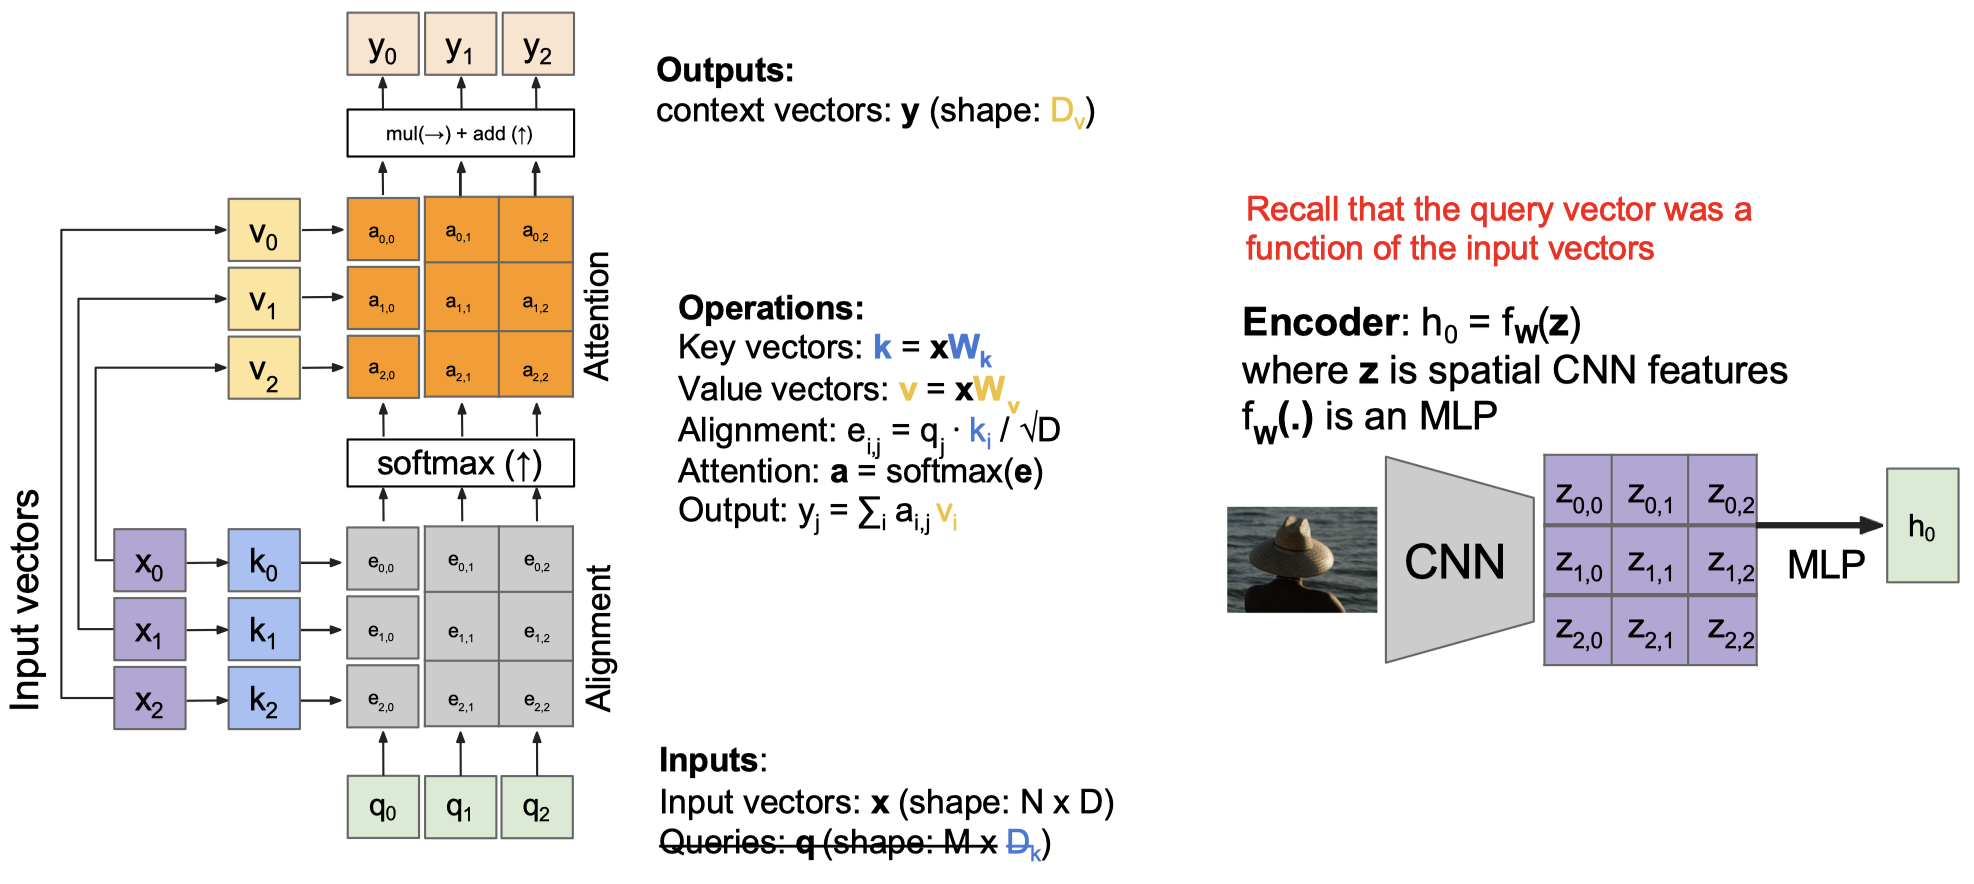
\includegraphics[width=0.8\textwidth]{figures/paralle_q.png}
    \caption{Self attention layer}
    \label{fig:paralle_q}
\end{figure}

根据相似度的计算方法, 可以发现 Self attention 是 Permutation equivariant 的, 就像 PointNet 一样.

但是这样就无法区别不同位置的 Token 了, 所以需要 Positional encoding

\begin{figure}[htbp]
    \centering
    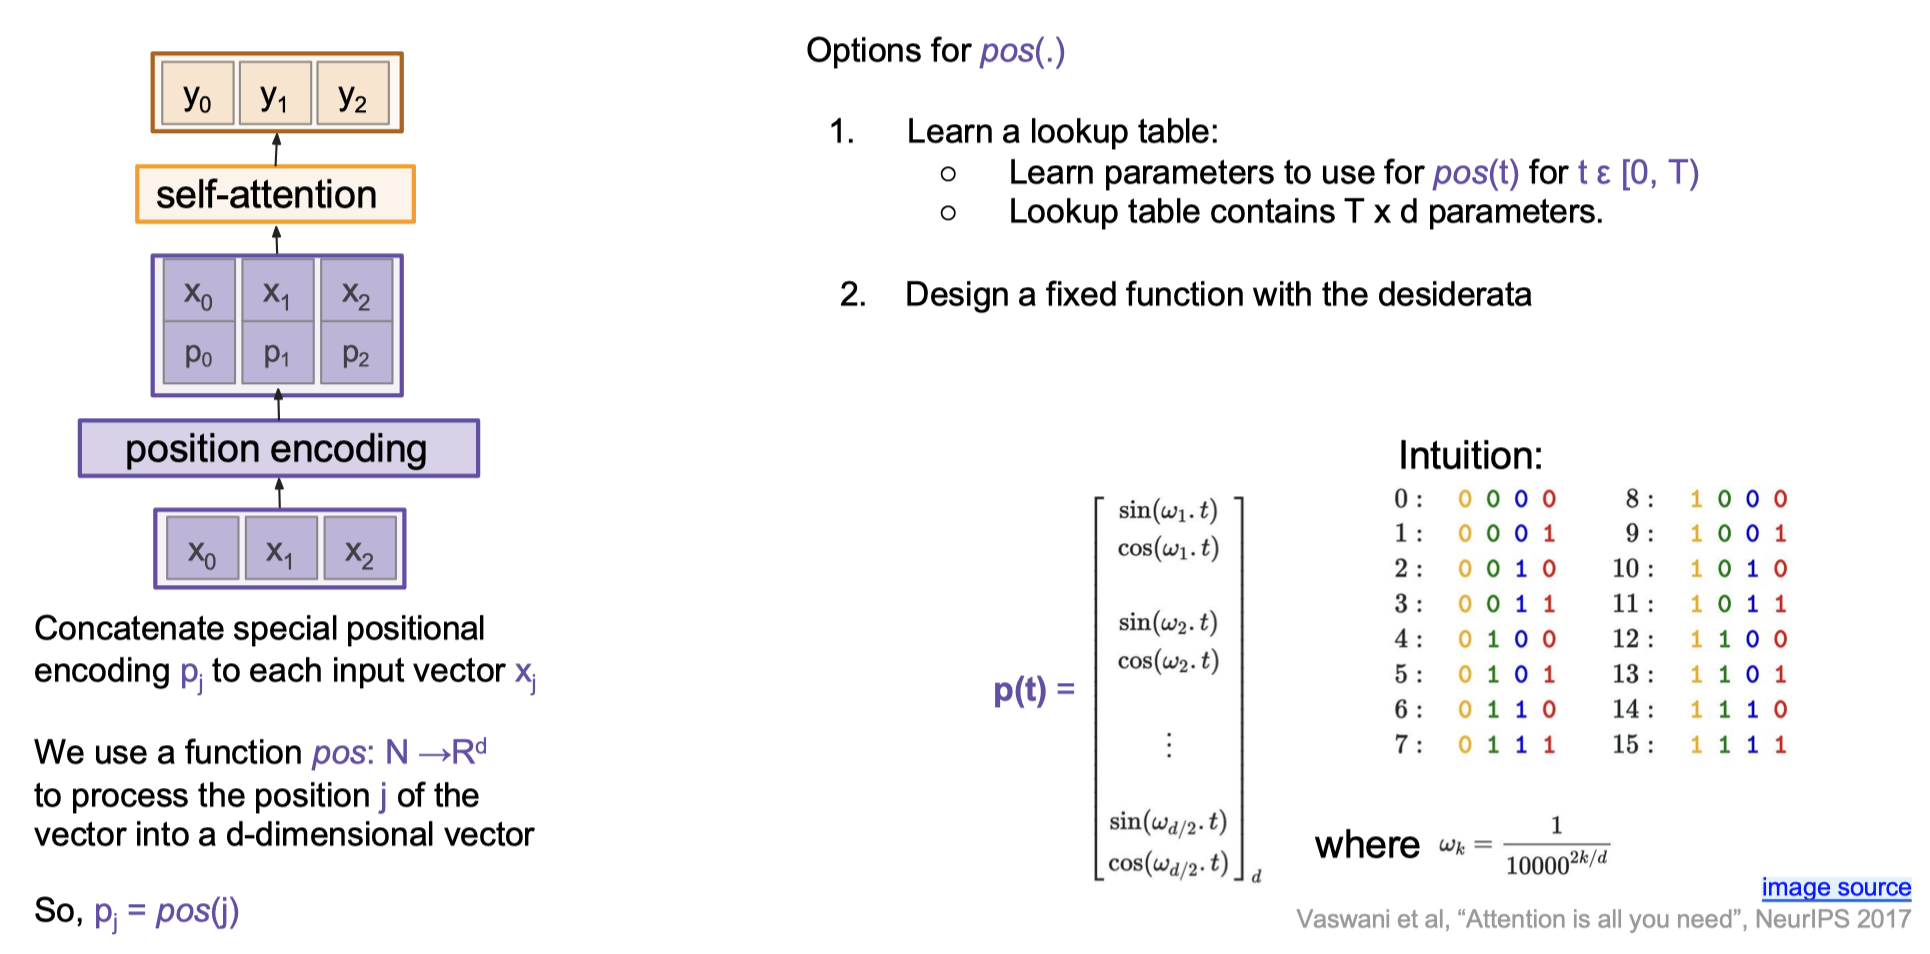
\includegraphics[width=0.8\textwidth]{figures/pos_encoding.png}
    \caption{Positional encoding}
    \label{fig:pos_encoding}
\end{figure}

不要小看 Positional encoding, 在处理大模型长序列的时候, Positional encoding 是核心技术点.

同时还不能让前面的 Query 对后面的 Key 进行查询, 所以需要mask.

为了提高多语义的能力, 可以加入 multi-head attention, 可以理解为不同的head可以学习到同一个 token 的不同意思,
在图像中可以理解为几千维的feature代表了一个像素区域, 现在需要把这些像素区域分开计算 attention, 会比一起计算有更好的表达能力.

\begin{figure}[htbp]
    \centering
    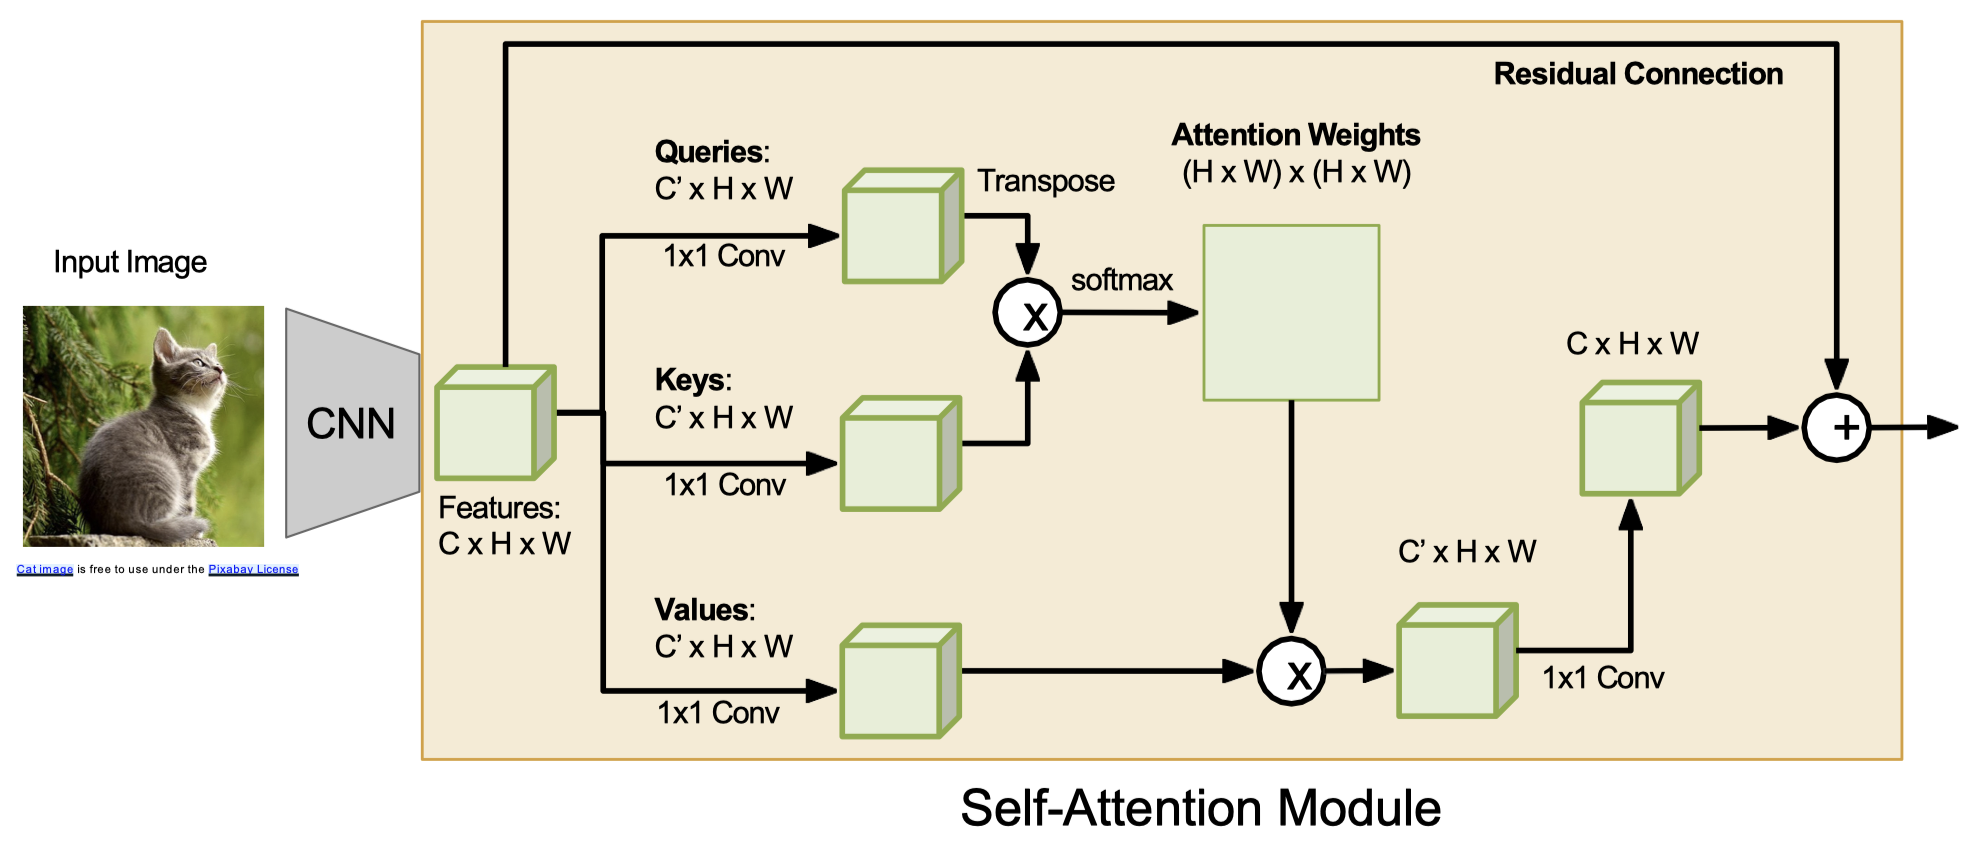
\includegraphics[width=0.8\textwidth]{figures/image_self_atten.png}
    \caption{CNN with Self-Attention}
    \label{fig:image_self_atten}
\end{figure}

一个例子: 图像上的自注意力机制

Transformer Encoder 和 Decoder 的区别: Encoder 是完全并行化的, Decoder 是有依赖的, 所以是串行的.

\subsection{Self-Supervised Learning (Pre-training)}

SimCLR design choices: large batch size 原因: 不希望在一些例子上over fit.

MAE, CLIP

Other examples: skip.

\subsection{Large Multi-modal Models}

BLIP

BLIP-2: Image Encoder 用CLIP based会好一些

InstructBLIP

Frozen: 发现 language model 不用train, 只用train vision Encoder

Flamingo

CLIP的问题:只能提取语义信息, 细节都丢失了.

交互是通往AGI的真正途径, 看了很多骑自行车的视频不代表我真的会了骑自行车
, embodied AI, 具身多模态大模型